%%
% TUM Corporate Design LaTeX Templates
% Based on the templates from https://www.tum.de/cd
%
% Feel free to join development on
% https://gitlab.lrz.de/tum-templates/templates
% and/or to create an issue in case of trouble.
%
% tum-presentation class for scientific talks, thesis presentations, ...
%
%%

%\documentclass[4to3]{tum-presentation}
%\documentclass[navsym]{tum-presentation}
%\documentclass[nothreeliner]{tum-presentation}
%\documentclass[handout,4on1]{tum-presentation}
%\documentclass[handout,2on1]{tum-presentation}
%\documentclass[handout]{tum-presentation}
\documentclass{tum-presentation}

\addbibresource{literature.bib}

\title[Shortened Title]{Clustering-Based Sentiment Analysis for Media Agenda Setting}
\subtitle{Opinion Lab Group 2.3}
\author{Wing Sheung Leung, Qiaoxi Liu}
%\institute[]{\inst{1} Department of Electrical and Computer Engineering,
%  Technical University of Munich (TUM)\\
%  \inst{2} Department of Informatics, Technical University of Munich (TUM)}
%\date{International Conference on Mostly Scientific Topics}

\footline{\insertshortauthor~| \inserttitle}

\begin{document}

\begin{frame}[noframenumbering]
  \titlepage
\end{frame}
\begin{frame}
  \frametitle{Milestones}
  \vspace{2cm}
 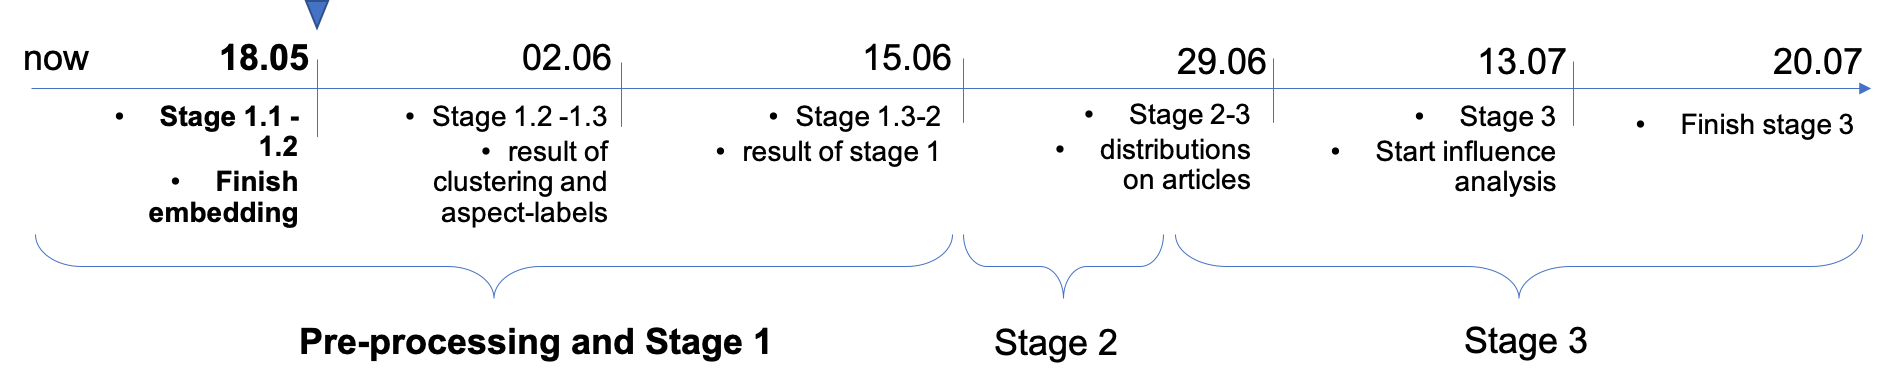
\includegraphics[width = \textwidth]{figures/timeline.png}
  
\end{frame}
\begin{frame}[t]
  \frametitle{Overview}
  \tableofcontents[sectionstyle=show,subsectionstyle=show,subsubsectionstyle=shaded]
\end{frame}




\subsection{1.2 Kmeans and Elbow Method}
\subsubsection{sklearn.cluster.MiniBatchKMeans}
\begin{frame}[fragile]
  \frametitle{Stage 1.2: sklearn.cluster.MiniBatchKMeans}
  \begin{lstlisting}
class KMeansClustering():
def __init__(self, k, X, is_mini_batch = True, plot_bar_chart = True):
  self.k = k
  self.X = np.array(X).reshape(len(X), 512)
  self.km = MiniBatchKMeans(n_clusters=k, init='k-means++', batch_size=3000, compute_labels=True).fit(self.X)
  \end{lstlisting}
  \begin{center}
    \begin{figure}[t]
      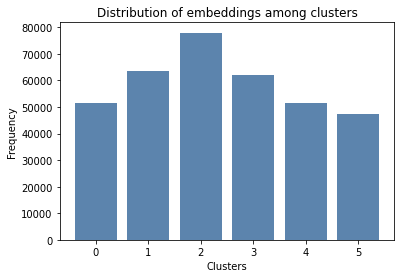
\includegraphics[width=0.35\textwidth]{images/6ks-overall-bar.png}
      \hspace{2cm}
      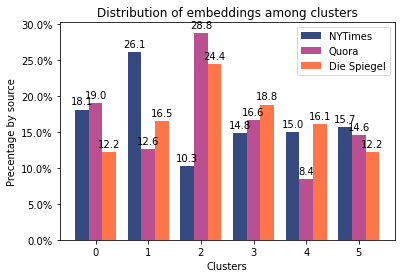
\includegraphics[width=0.35\textwidth]{images/6ks-grouped-bar.png}
      \caption{Example of distribution of embeddings of all tokenized sentences from the three sources among 6 clusters}
    \end{figure}
  \end{center}
\end{frame}
\begin{frame}[fragile]
  \frametitle{Stage 1.2: sklearn.cluster.MiniBatchKMeans}
  \framesubtitle{Why MiniBatchKmeans instead of original sklearn.cluster.KMeans}
  \begin{description}
    \item XLING sentence level embeddings is generated in 512 dimensions for each tokenized sentence by NLTK.
  \end{description}
  \begin{figure}[t]
    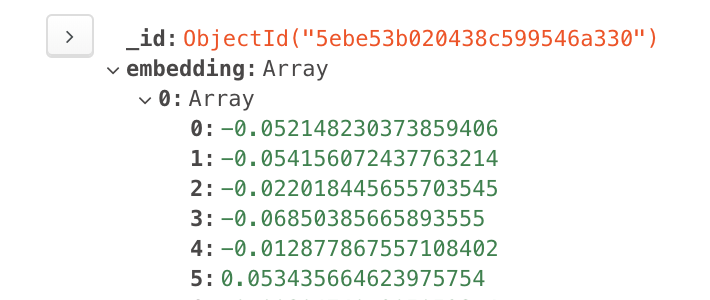
\includegraphics[width=0.35\textwidth]{images/embedding-sample-1.png}
    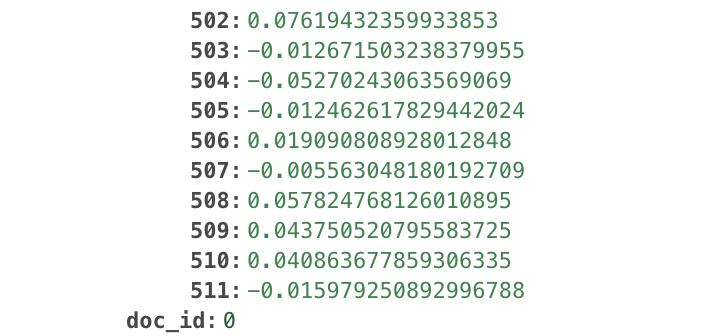
\includegraphics[width=0.35\textwidth]{images/embedding-sample-2.png}
    \caption{XLING embedding output for a sample sentence. Left: First 6 dimensions. Right: Last 10 dimensions}
  \end{figure}
  \small
  \begin{table}[t]
    \begin{tabular}{lcc}
    \hline
      Source & Embedding JSON size & Original corpus size\\ \hline
      New York Times & 827 MB & 55.9 MB\\
      Quora & 638 MB & 15.9 MB\\
      Die Speigel & 2.3 GB & 131 MB\\
    \hline
    \end{tabular}
    \caption{Embeddings generated are greatly larger then the original corpus size}
  \end{table}
\end{frame}

\subsubsection{Elbow Method for determining optimal k}
\begin{frame}[fragile]
  \frametitle{Stage 1.2: Elbow Method for determining optimal k}
  \begin{lstlisting}
K = range(2, 21)
for k in K:
  model = KMeansClustering(k, X)
  distortions.append(model.km.inertia_)
  \end{lstlisting}
  \begin{center}
    \begin{figure}[t]
      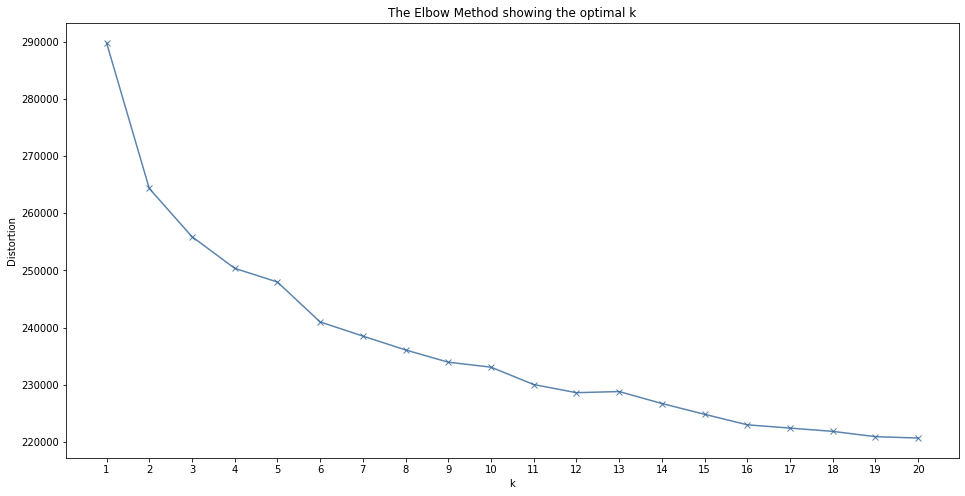
\includegraphics[width=0.33\textwidth]{images/elbow-1.png}
      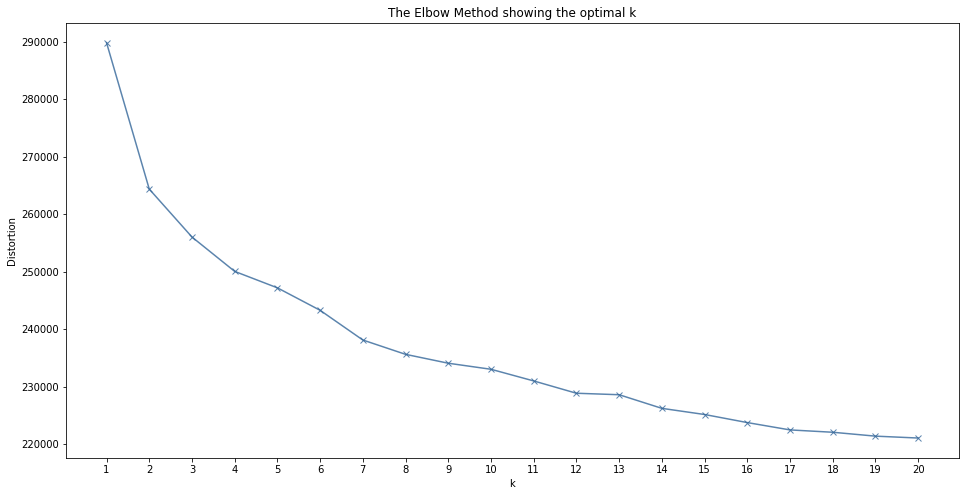
\includegraphics[width=0.33\textwidth]{images/elbow-2.png}
      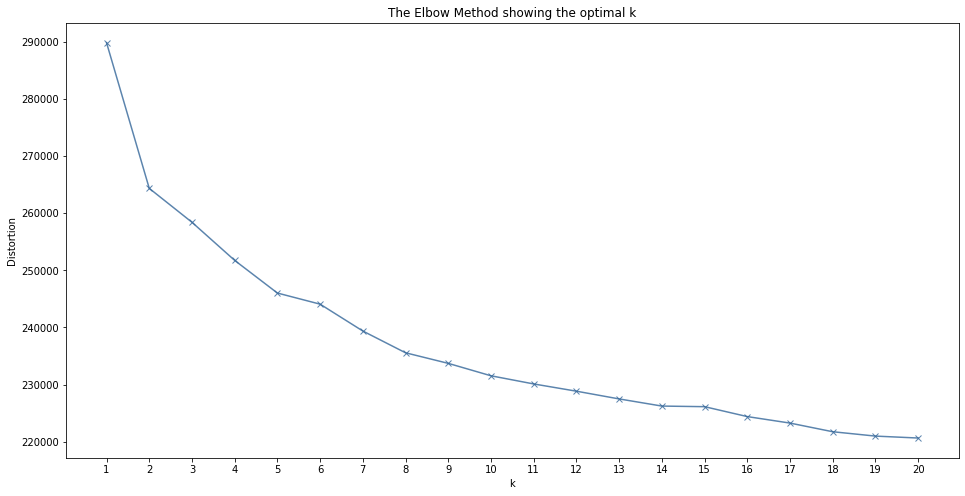
\includegraphics[width=0.33\textwidth]{images/elbow-3.png}
      \caption{After few epochs of K-Means clustering, there is no distinguishable elbow of the curve for determination of optimal k}
    \end{figure}
  \end{center}
\end{frame}

\begin{frame}[fragile]
  \frametitle{Stage 1.2: sklearn.cluster.MiniBatchKMeans}
  \framesubtitle{Why MiniBatchKmeans instead of original sklearn.cluster.KMeans}
  \begin{description}
    \item  Just loading all sentence embeddings in Google Colaboratory, 6.36 GB out of the given 12.72 GB RAM had already been used up. 
  
    \item  MiniBatchKMeans is faster and helps to prevent the session from crushing, however, gives slightly different results.
  \end{description}


  \begin{figure}[t]
    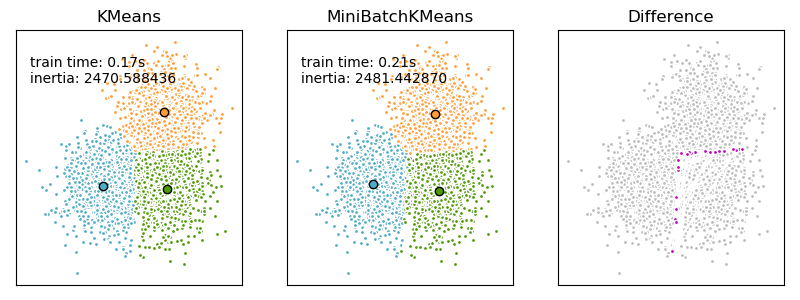
\includegraphics[width=0.60\textwidth]{images/sphx_glr_plot_mini_batch_kmeans_001.png}
    \caption{Extracted from scikit-learn; Data points classified differently are shown as purple points in 'Difference' block}
    \url{https://scikit-learn.org/stable/auto_examples/cluster/plot_mini_batch_kmeans.html}
  \end{figure}
\end{frame}


\subsubsection{AIC for determining optimal k}
\begin{frame}[fragile]
  \frametitle{Stage 1.2: AIC for determining optimal k}
  \begin{lstlisting}
def get_AIC(self):
    k, m = self.km.cluster_centers_.shape # dimension of centroids
    D = self.km.inertia_ # within-cluster sum of square distances, residual sum of squares 
    AIC = D + 2 * m * k
    return AIC
  \end{lstlisting}
  \begin{center}
    \begin{figure}[t]
      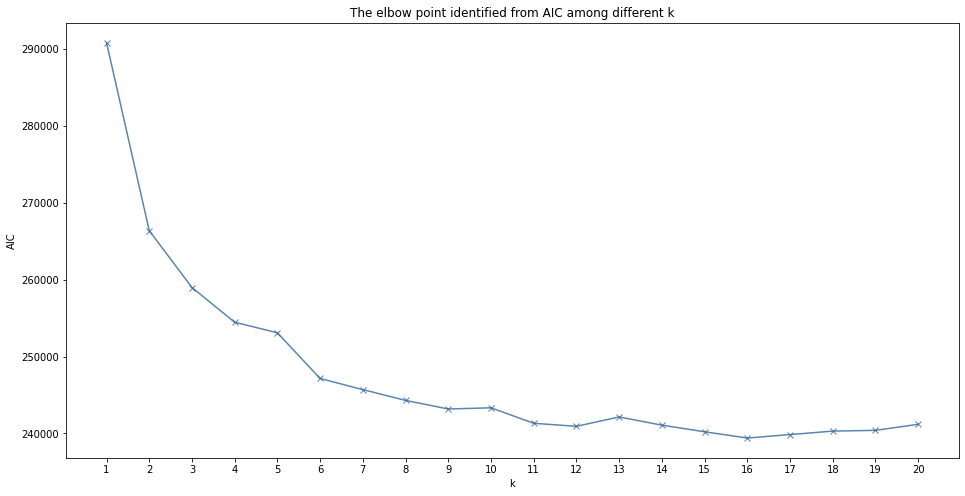
\includegraphics[width=0.33\textwidth]{images/AIC-1.png}
      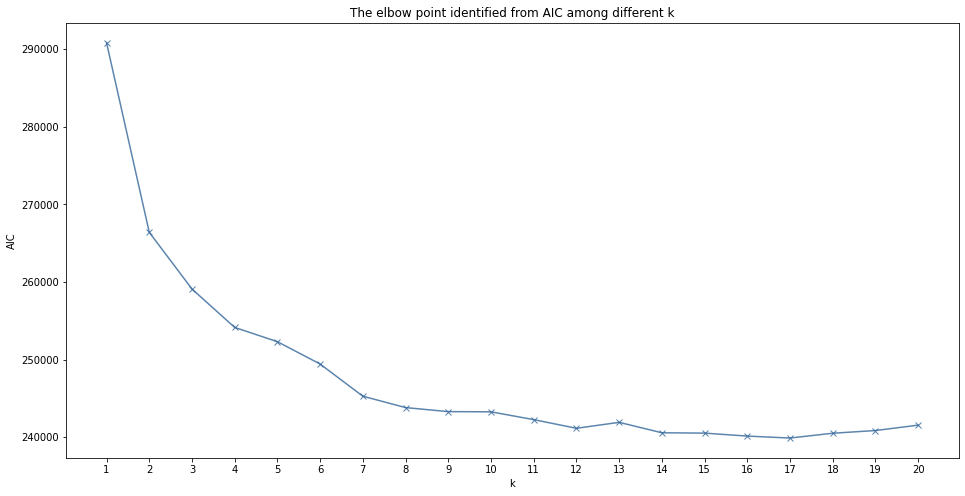
\includegraphics[width=0.33\textwidth]{images/AIC-2.png}
      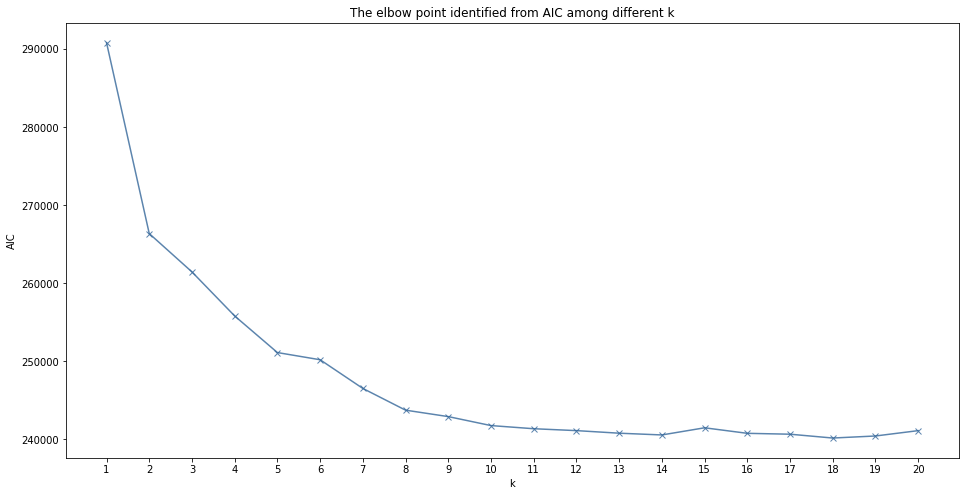
\includegraphics[width=0.33\textwidth]{images/AIC-3.png}
      \caption{For those epochs, AIC curves more or less follow the trends in elbow method, but it is more feasible to see that the curves become more steady from k larger than 7 or 8.}
    \end{figure}
  \end{center}
\end{frame}
\subsubsection{BIC for determining optimal k}
\begin{frame}[fragile]
  \frametitle{Stage 1.2: BIC for determining optimal k}
  \begin{lstlisting}
def get_BIC(self):
  k, m = self.km.cluster_centers_.shape # dimension of centroids
  n = self.n
  D = self.km.inertia_ # within-cluster sum of square distances, residual sum of squares 
  BIC = D + 0.5 * m * k * np.log(n)
  return BIC
  \end{lstlisting}
  \begin{center}
    \begin{figure}[t]
      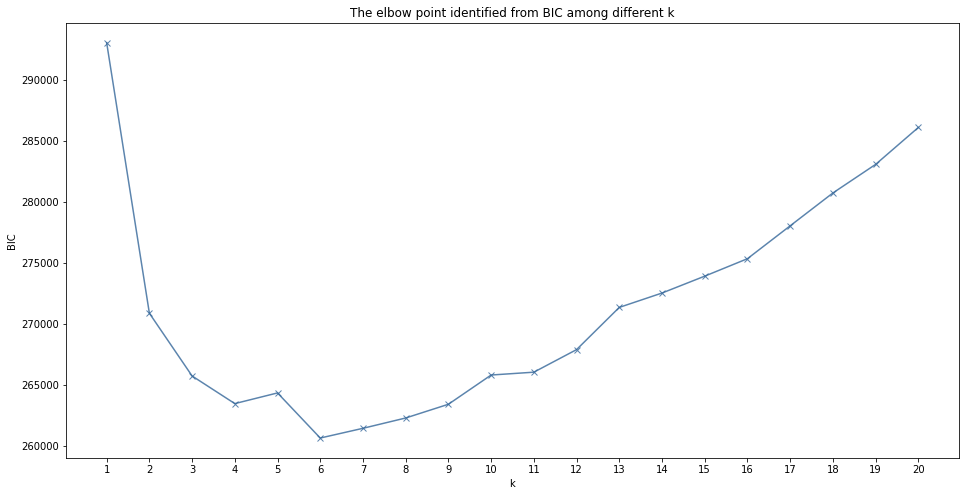
\includegraphics[width=0.33\textwidth]{images/BIC-1.png}
      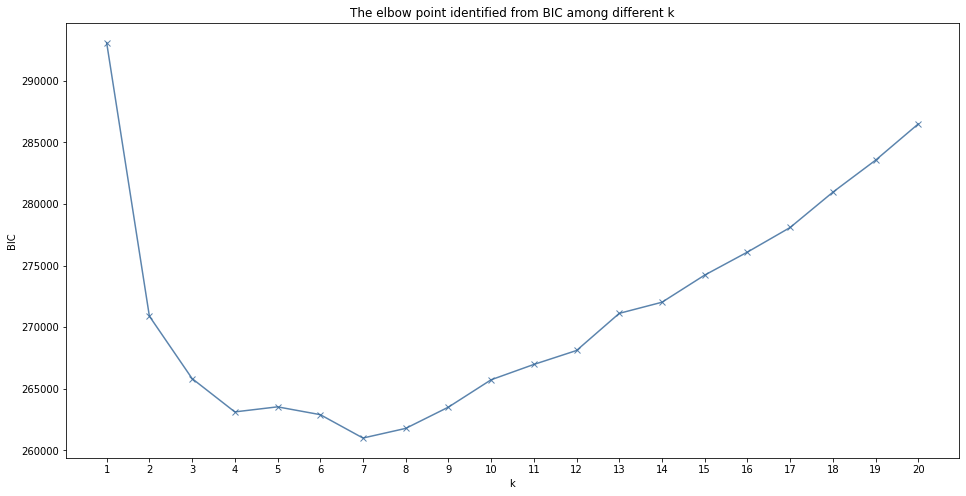
\includegraphics[width=0.33\textwidth]{images/BIC-2.png}
      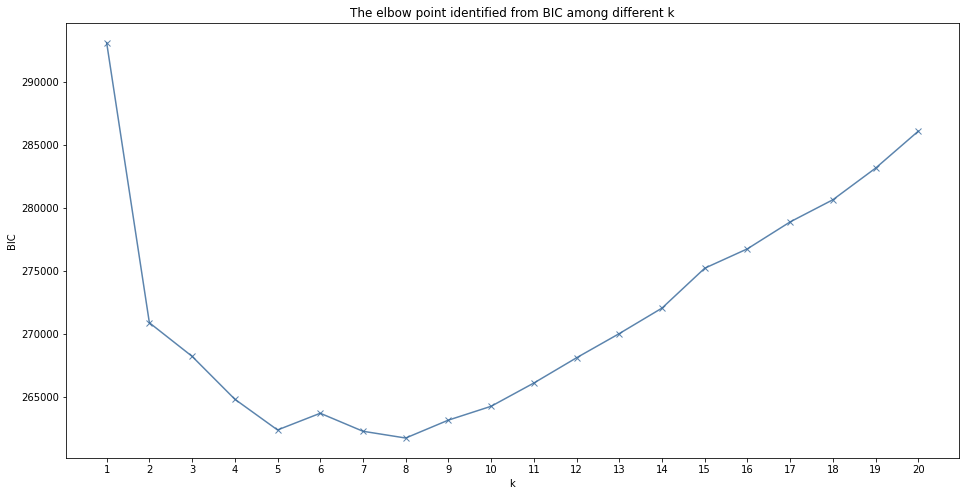
\includegraphics[width=0.33\textwidth]{images/BIC-3.png}
      \caption{For those epochs, 5 to 8 are the potential candidates for optimal k}
    \end{figure}
  \end{center}
\end{frame}
\subsubsection{Determination of suitable k by looking at top n words in each potential clusters}
\begin{frame}[fragile]
  \frametitle{Stage 1.2: Determination of suitable k by looking at top n words in each potential clusters}
  \end{frame}

  \subsubsection{Clustering results}
  \begin{frame}[fragile]
    \frametitle{Clustering results (different k)}
    
      Under each k, there is a cluster without NYtimes sentence.
      
      \begin{center}
        \begin{figure}[t]
          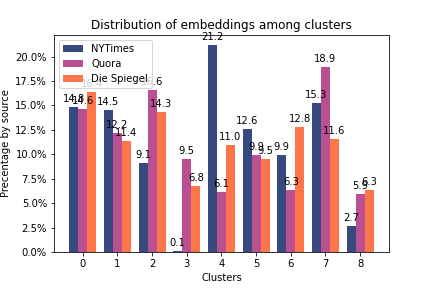
\includegraphics[width=0.19\textwidth]{figures/kmean-output_9ks-grouped-bar.png}
          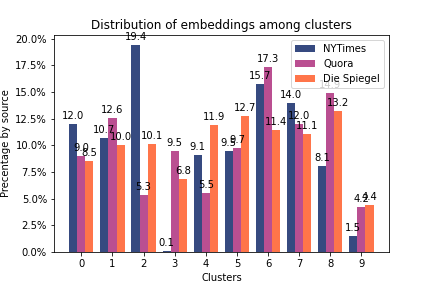
\includegraphics[width=0.19\textwidth]{figures/kmean-output_10ks-grouped-bar.png}
          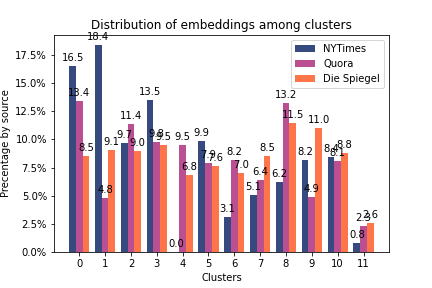
\includegraphics[width=0.19\textwidth]{figures/kmean-output_12ks-grouped-bar.png}
          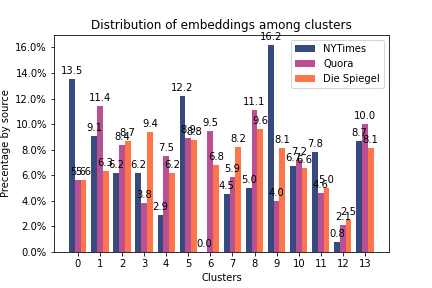
\includegraphics[width=0.19\textwidth]{figures/kmean-output_14ks-grouped-bar.png}
          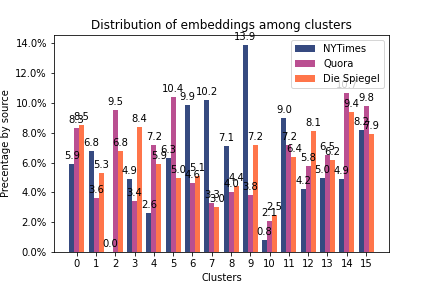
\includegraphics[width=0.19\textwidth]{figures/kmean-output_16ks-grouped-bar.png}
          \caption{distribution for k=9, 10, 12, 14, 16}
        \end{figure}
      \end{center}
    \begin{center}
      \begin{figure}[t]
        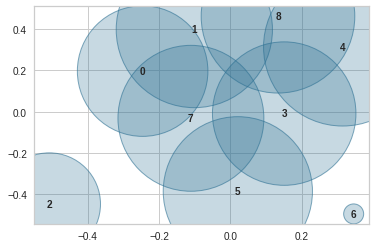
\includegraphics[width=0.19\textwidth]{figures/k09.png}
        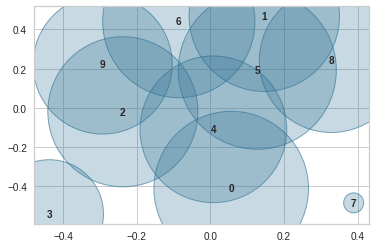
\includegraphics[width=0.19\textwidth]{figures/k10.png}
        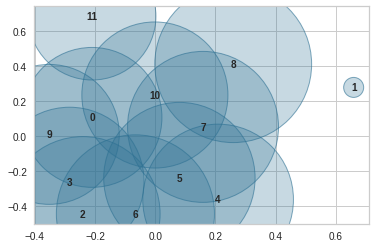
\includegraphics[width=0.19\textwidth]{figures/k12.png}
        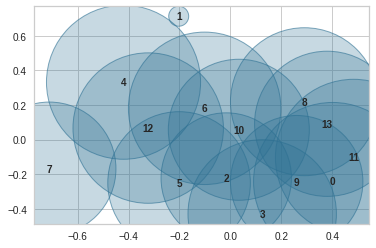
\includegraphics[width=0.19\textwidth]{figures/k14.png}
        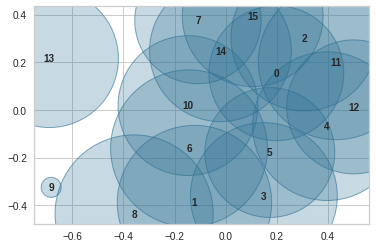
\includegraphics[width=0.19\textwidth]{figures/k16.png}
        
      \end{figure}
    \end{center}
  
    \end{frame}

    \begin{frame}[fragile]
      \frametitle{tokenizing, stemming and stopwords}
      \begin{description}
        \item 1. tokenizer chosen from ... 
        \item 2. stemming : (using existing libraries ) customized list for both languages
        \item for example: farmer/farming/farm/  product/produce/production/ 
        \item 3. stopwords : also using libararies + customized list for both languages
      \end{description}

     
      \end{frame}
    \begin{frame}[fragile]
      \frametitle{Top words (frequencies / tfidf)}
strategy 1: delete the repeated one which appear more than a ratio (0.5)

      \begin{center}
        \begin{figure}[t]
          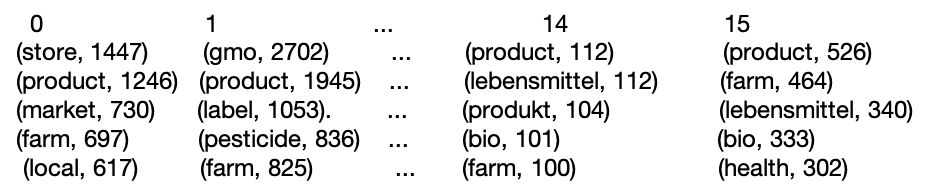
\includegraphics[width=0.6\textwidth]{figures/naivetopwords.png}
        \end{figure}
      \end{center}
      strategy 2: clarity scores
      \end{frame}
    \subsubsection{Clustering wordclouds}
    \begin{frame}[fragile]
      \frametitle{Wordclouds k = 13}

        \begin{center}
          \begin{figure}[t]
            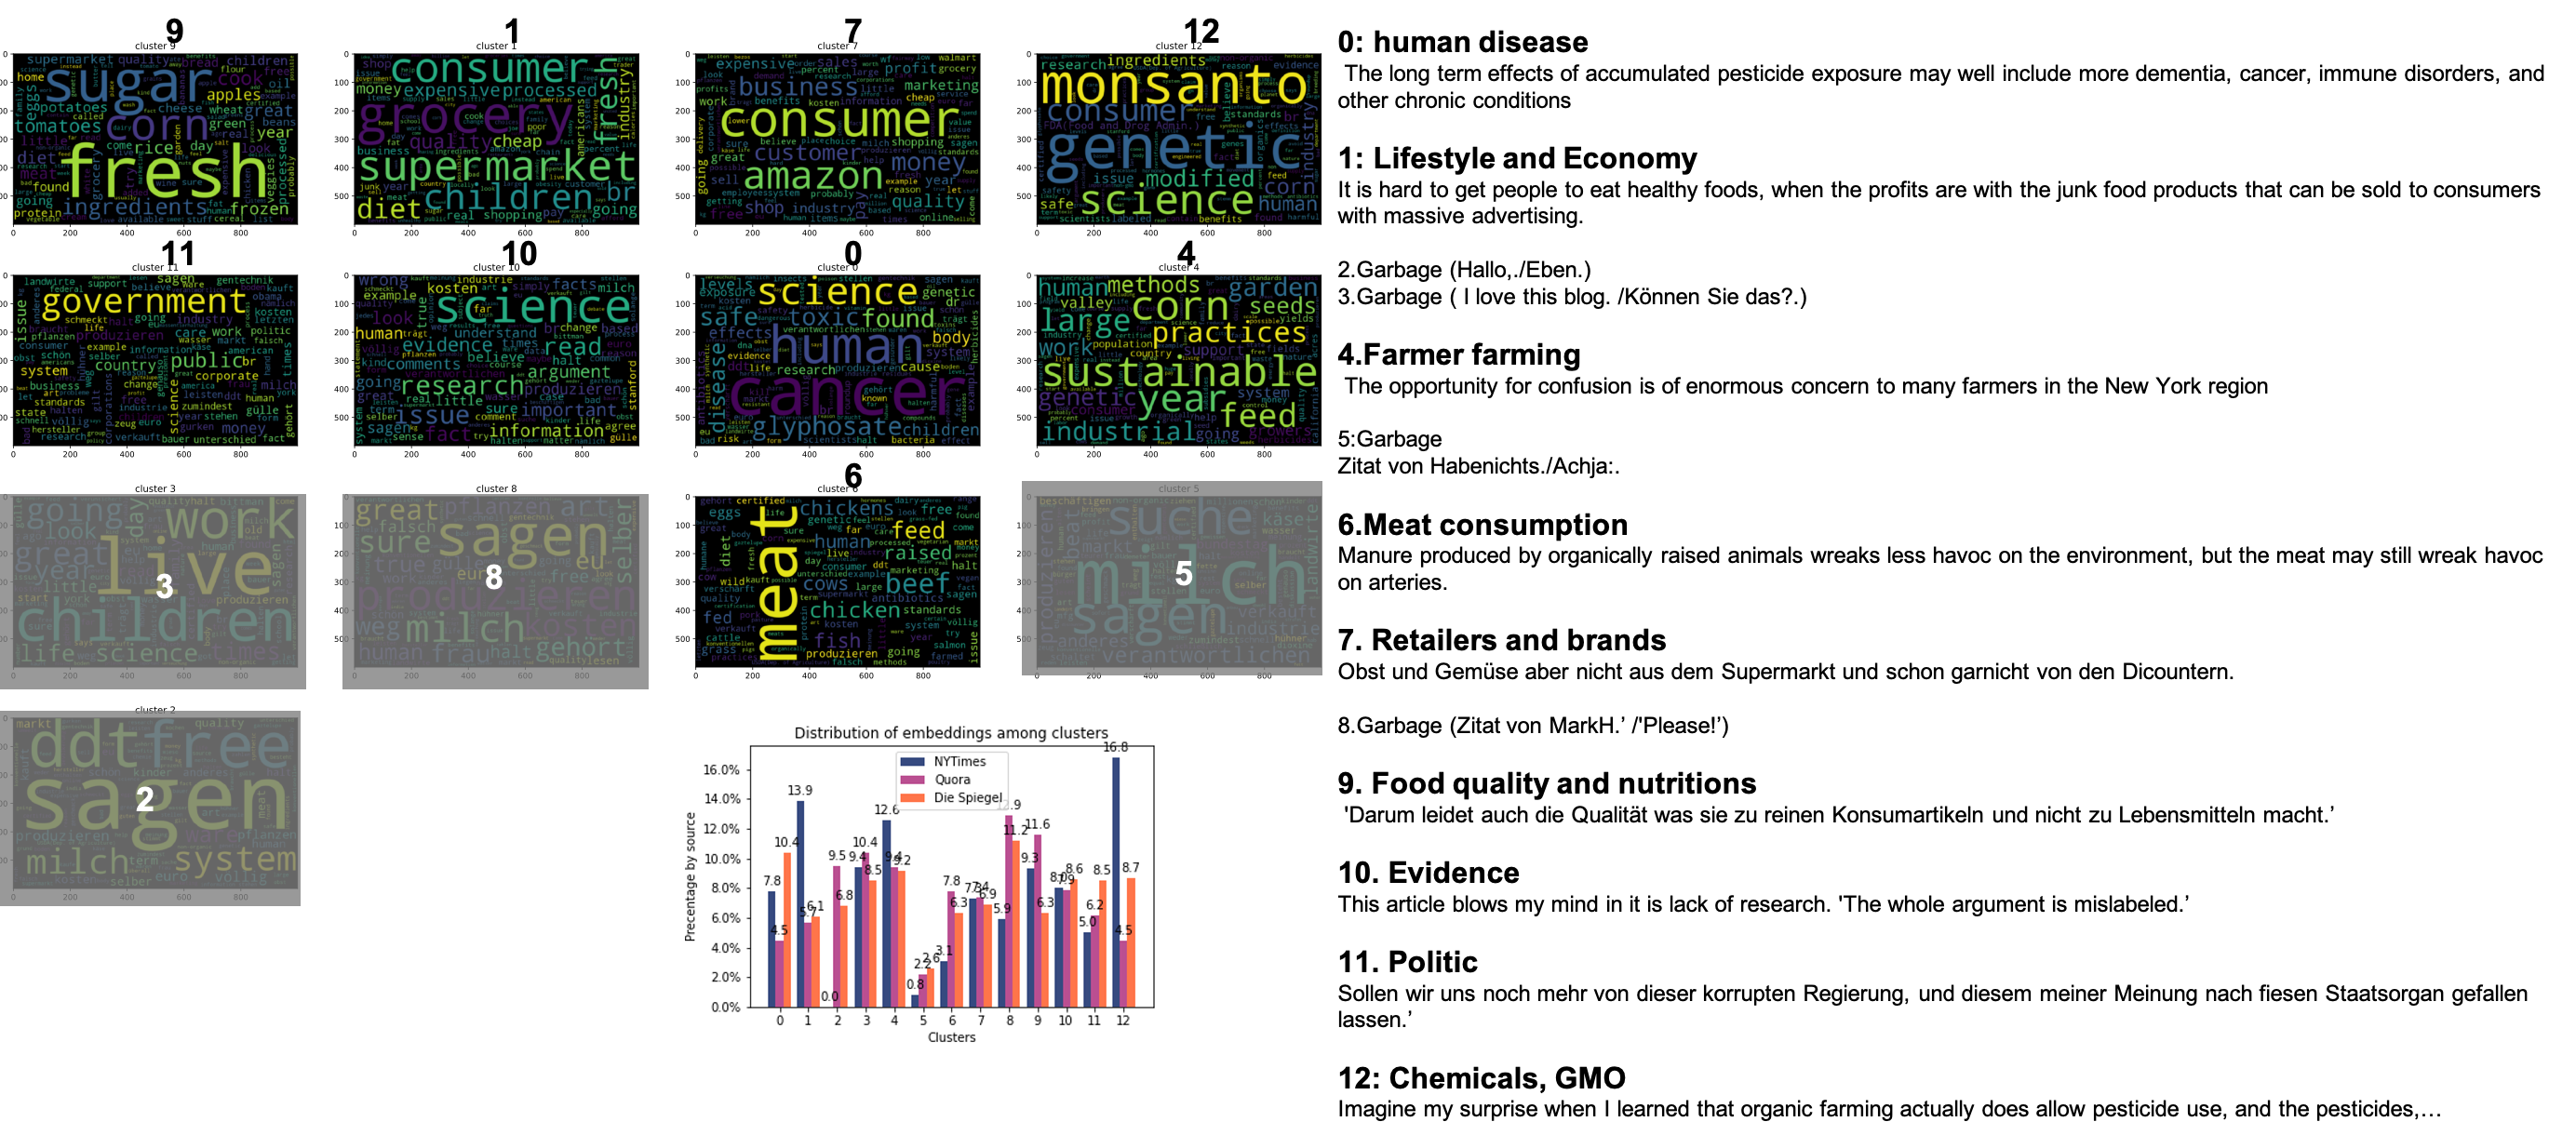
\includegraphics[width=0.9\textwidth]{figures/example13.png}

          \end{figure}
        \end{center}
      
    
      \end{frame}
\section{Future Plan}
\begin{frame}
  \frametitle{Next steps...}
  \begin{description}
    \item 1. confirm the ideal k
    \item 2. sentiment classification
  \end{description}
 
\end{frame}

\end{document}
